% !TeX root = ../Noctua_Pflichtenheft.tex

% Chapter7
\chapter{Schnittstellen} \label{chapter:schnittstellen}

Die Schnittstelle des Projektes, die den Benutzer am meisten betrifft, ist die der \gls{bts}. Sie soll zur Erleichterung der Bedienung eine simple grafisches Benutzerschnittstelle (GUI) aufweisen, �ber die s�mtliche Funktionen verf�gbar sind. Abbildung \ref{fig:bts_gui} stellt eine m�gliche GUI der Backtesting-Software dar, �ber die die historischen Daten als File ausgew�hlt und eingelesen werden k�nnen und der Algorithmus ebenso.\\

\begin{figure}[h]
	\centering
		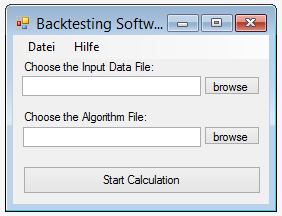
\includegraphics[width=0.5\textwidth]{graphics/schnittstellen/bts_gui.png}
	\caption[Backtesting-Software Steuerungs-GUI]{Backtesting-Software Steuerungs-GUI zur Auswahl historischer Daten und eines Algorithmus}
	\label{fig:bts_gui}
\end{figure}

	Die \gls{bts} soll  die berechneten Kennzahlen des implementierten Handelssystems ausgeben und diese so �bersichtlich anzeigen, dass sie dem Anwender folglich als Vergleichswerte dienen. F�r diesen Zweck ist eine �bersichtliche tabellarische Auflistung bestens geeignet. Diese Kennwerte k�nnen mit der Software als Textdatei gespeichert werden, um etwaige Berechnungen durchzuf�hren oder die Kennzahlen mit anderen Algorithmen zu vergleichen.\\
\\
Neben der Benutzungsschnittstelle spielt au�erdem noch die Schnittstelle zwischen der \gls{bts} und dem Algorithmus eine Rolle, genauer gesagt, wie dieser an die \gls{bts} angebunden oder integriert wird.\\
	Der Algorithmus soll eine eigenst�ndige Komponente sein, die modular aufgebaut wird, damit sie einfach ausgetauscht werden kann. Daher �bernimmt die \gls{bts} die Aufgabe, dieses Modul anzuwenden. Aus der Sicht des Benutzers ist der Algorithmus eine Datei, die in der Oberfl�che der \gls{bts} ausgew�hlt wird und auf diese Art und Weise auch gewechselt werden kann.\\
	F�r Anwender der \gls{bts} wird eine Dokumentation angefertigt, die diese Schnittstelle zwischen \gls{bts} und Algorithmus genau beschreibt und so dem Programmierer erm�glicht seinen Algorithmus der notwendigen Architektur nach zu programmieren. Der schematische Aufbau eines Algorithmus, der von der \gls{bts} akzeptiert wird, ist somit genau als Softwarebestandteil und ebenso in der Dokumentation vorgegeben, um fehlerhafte Algorithmen nicht auszuf�hren und deren Entstehung durch Information der Entwicklerseite �berhaupt zu verhindern. Die Schnittstelle spezifiziert die konkrete Implementierung von Kauf- und Verkaufsignalen zu bestimmten Zeitpunkten auf Algorithmusseite, damit die \gls{bts} diese zur berechnung umsetzen kann. In die andere Richtung ist spezifiziert, wie im Algorithmus auf die historischen Kursdaten, die die \gls{bts} bereitstellt, zugegriffen werden kann.\\
\\
/B010/ \textbf{Algorithmusintegration}\\
Der Benutzer soll den Algorithmus in der \gls{bts} als Datei aus dem Dateisystem �ber eine GUI ausw�hlen k�nnen.\\
\\
/B020/ \textbf{Kenndatenanzeige}\\
Kenndaten des Algorithmus sollen dem Benutzer in tabellarischer Form �bersichtlich gegliedert angezeigt werden.\\
\\
/B030/ \textbf{Datenspeicherung}\\
S�mtliche berechneten Kenndaten sollen �ber die GUI in menschenlesbarer Form als Textdatei abgespeichert werden k�nnen.\\